\chapter{Tecnologías relacionadas con los componentes}\label{ch:tecnologias-relacionadas-con-los-componentes}

En este capítulo se abordará el desarrollo de las
diferentes tecnologías que permiten a \textit{JAMS}
tener una estructura modular, haciendo que los
componentes puedan modificarla para incluir o modificar
diferentes características.
Cabe destacar que estas tecnologías no solo son usadas
por los componentes, sino que \textbf{el propio \textit{JAMS}}
aprovecha sus virtudes para proporcionar características
dentro del programa principal.


\section{Gestores}\label{sec:gestores}

Toda la arquitectura de la aplicación está basada en \textbf{gestores}.
Un gestor se puede definir como un conjunto de elementos que las herramientas pueden usar.
\textit{JAMS} proporciona tres tipos básicos de gestores:
\begin{itemize}
    \item \textbf{Gestores normales}: implementados por la clase \textit{Manager}.
    Contienen una lista de elementos sin ninguna jerarquía.
    \item \textbf{Gestores con valor por defecto}: actúa como un gestor normal, con la
    diferencia que uno de sus valores es el valor por defecto.
    Estos gestores heredan de la clase \textit{DefaultValuableManager}.
    \item \textbf{Gestores con valor seleccionado}: actúan como un gestor con valor por defecto,
    pero con uno de los elementos seleccionado.
    Cuando el elemento seleccionado se elimina, el elemento por defecto queda seleccionado.
    Estos gestores heredan de la clase \textit{SelectableManager}.
\end{itemize}

\subsection{Proveedores}\label{subsec:proveedores}

Cada elemento guardado en un gestor \textbf{está asociado al proveedor que lo proporciona}.
Un proveedor puede ser un componente o el propio \textit{JAMS}.
Cuando un proveedor se desvincula de la aplicación, todos los elementos proporcionados
por el proveedor son eliminados de los gestores.
Este diseño es una de las principales razones por las que la carga y descarga de
componentes es viable en \textit{JAMS}.
Al tener todos los elementos de correctamente etiquetados, \textit{JAMS}
puede retirar los elementos de un componente cuando éste se
descarga con una simple llamada a cada gestor.

\subsection{Registro}\label{subsec:registro}

El registro es un \textbf{elemento estático dentro de la aplicación}.
Se puede considerar un \textbf{gestor de gestores}.
En el registro se pueden recuperar, añadir, eliminar o modificar gestores.
Igual que los gestores normales, cuando un proveedor se desvincula de la aplicación,
todos los gestores proporcionados por el proveedor son eliminados del registro.

 \textit{JAMS} permite separar los gestores en dos tipos:
\textbf{gestores primarios} y \textbf{gestores secundarios}.
Los gestores primarios son fácilmente accesibles cuando se busca un gestor por tipo
usando métodos como $Manager.of(Type.class)$.
Solo puede existir un gestor primario por tipo.
Para buscar gestores secundarios, se debe proveer el nombre del gestor explícitamente.

\subsection{Uso de los gestores}\label{subsec:uso-de-los-gestores}

Como ya se ha presentado, un componente puede añadir, eliminar
y modificar \textbf{los elementos de los gestores y los gestores en sí}.
Definir nuevos gestores es muy sencillo: simplemente se debe crear
una nueva clase que extienda a $Manager$ o a alguno de sus hijos,
como se puede ver en la figura \ref{fig:manager-definition}.

\begin{figure}[h]
    \centering
    \begin{lstlisting}[frame=single,label={lst:manager-definition},language=Kotlin]
data class MyElement(
    private val name: String,
    private val provider: ResourceProvider
) : ManagerResource {
    override fun getName() = name
    override fun getResourceProvider() = provider
}

class MyManager(provider: ResourceProvider) : Manager<MyElement>(
    provider,
    "my-manager",
    MyElement::class.java,
    false
) {
    override fun loadDefaultElements() {}
}
    \end{lstlisting}
    \caption{Definición de un un gestor}
    \label{fig:manager-definition}
\end{figure}

 Una vez definido el gestor, este se debe \textbf{registrar}.
Para ello, se debe de acceder al registro.
Una vez registrado, cualquier componente podrá acceder al
gestor empleando los métodos proporcionados por el propio \textit{JAMS},
como se puede observar en la figura \ref{fig:manager-use}.

\begin{figure}[h]
    \centering
    \begin{lstlisting}[frame=single,label={lst:manager-use},language=Kotlin]
class MyPlugin : Plugin() {

    private fun registerAndUseManager() {
        Jams.REGISTRY.registerPrimary(MyManager(this))

        val manager = Manager.of(MyElement::class.java)
        manager.add(MyElement("Test element", this))

        manager.filter { it.name.startsWith("T") }
            .forEach { println(it.name) }
    }
}
    \end{lstlisting}
    \caption{Definición de un un gestor}
    \label{fig:manager-use}
\end{figure}


\section{Eventos}\label{sec:eventos}

\textit{JAMS} incluye un sistema de eventos que permite informar
de sucesos entre componentes de la aplicación.
Este sistema está profundamente inspirado en el sistema de eventos
utilizado por la comunidad de \textit{Minecraft}
en proyectos como \textit{Spigot}\cite{SPIGOT}
o \textit{Sponge}\cite{SPONGE}, y puede considerarse una evolución descentralizada
de esta tecnología.

\subsection{Emisores de eventos}\label{subsec:emisores-de-eventos}

Los emisores de eventos son los encargados de transmitir
eventos a los elementos que los escucha.
Puede considerarse un \textbf{canal} por el cual diferentes creadores
de eventos pueden transmitir diferentes tipos de eventos
que los elementos escuchando pueden recibir.

 Un emisor de eventos está representado por la interfaz $EventBroadcast$.
Esta interfaz es implementada por cualquier elemento que quiera ser
usado para registrar escuchas.
Los gestores, los componentes o el propio \textit{JAMS} implementan
un emisor por defecto.
La clase $SimpleEventBroadcast$ contiene una implementación de $EventBroadcast$
que se puede utilizar como superclase.

\subsection{Definir escuchas}\label{subsec:definir-escuchas}

Las escuchas son \textbf{métodos no estáticos anotados con la anotación @Listener}.
Estos métodos solo tienen un parámetro que pide un elemento que extienda la clase
$Event$ y deben devolver $void$.
Este método, después de ser registrado en un gestor de idiomas,
se ejecutará cuando un nuevo idioma sea añadido al gestor.
Un ejemplo de escucha puede observarse en la figura \ref{fig:listener}.

\begin{figure}[h]
    \centering
    \begin{lstlisting}[frame=single,label={lst:listener},language=Kotlin]
@Listener
fun onLanguageRegister(
    event: ManagerElementRegisterEvent.After<Language>
) {
    println("New language available! ${event.element.name}")
}
    \end{lstlisting}
    \caption{Objeto registrando un evento en el emisor general de \textit{JAMS}}
    \label{fig:listener}
\end{figure}

 A diferencia de otros sistemas de eventos similares,
el sistema de eventos de \textit{JAMS} permite usar \textbf{eventos genéricos}.
Un ejemplo es el caso anterior, donde el método pide un elemento de tipo
$ManagerElementRegisterEvent.After<Language>$.
Si el emisor al que está registrado emite un evento de tipo
$ManagerElementRegisterEvent.After<Theme>$, la escucha no será invocada.

 Un evento puede extender la clase de otro evento.
Esto permite generar una jerarquía de eventos.
Una escucha que pide un cierto tipo de evento se ejecutará siempre que dicho evento o uno de sus hijos ocurra.
Si una escucha pide el evento $Event$, su método se ejecutará siempre que un evento ocurra.

 Algunos eventos implementan la interfaz $Cancellable$, lo cual permite cancelar el evento.
Las escuchas restantes no serán llamadas cuando un evento es cancelado salvo que se defina lo contrario
en la etiqueta $@Listener$.

\subsection{Registrar escuchas}\label{subsec:registrar-escuchas}

Una vez un objeto tenga definidas todas sus escuchas, estas
se puede registrar en uno o varios emisores de eventos.
Para ello se debe llamar al método $registerListeners$ del
emisor deseado, tal y como se muestra en la figura \ref{fig:event-registration}.

\begin{figure}[h]
    \centering
    \begin{lstlisting}[frame=single,label={lst:event-registration-use},language=Kotlin]
class ObjectWithListeners {

    init {
        Jams.getGeneralEventBroadcast().registerListeners(
            /* instance = */ this,
            /* useWeakReferences = */ true
        )
    }

    @Listener
    private fun onEvent(event: Event) {
        println("I received a new event! $event")
    }

}
    \end{lstlisting}
    \caption{Objeto registrando un evento en el emisor general de \textit{JAMS}}
    \label{fig:event-registration}
\end{figure}

 El método de registro pide dos simples variables: el objeto
con las escuchas y si se deben usar \textbf{referencias débiles}.
Esta última opción permite a los objetos eliminarse de la memoria
cuando ya no sean necesarios, incluso aunque tengan escuchas registradas.
Estas escuchas \textbf{serán eliminadas del emisor automáticamente} si no existe
ninguna referencia al objeto (sin contar la del propio emisor).
Esto permite desarrollar componentes de una manera \textbf{muy sencilla}:
combinado con el sistema de proveedores, las referencias débiles
de las escuchas evita que la aplicación mantenga elementos de un
componente cuando este se desinstala.

 Por último, cabe destacar que el método de registro
busca todos los métodos de escucha de un objeto,
\textbf{buscando también en los métodos de las clases padres}.
Esto permite heredar funcionalidades de objetos ya programados
de manera sencilla.
Si el desarrollador desea registrar un único método puede hacerlo
con los métodos proporcionados, pero para ello se requieren
conocimientos de la librería \textit{reflection} de \textit{Java}.


\section{Tareas}\label{sec:tareas}

Las tareas son elementos muy importantes dentro de una aplicación
de escritorio.
Estas consisten en \textbf{funciones que ejecutan una tarea de manera
asíncrona al hilo principal} de la aplicación, devolviendo un
resultado al finalizar su ejecución.
\textit{Java} proporciona diversas maneras de gestionar
las tareas dentro de una aplicación, y \textit{JavaFX}
también implementa su propia solución.
Es por eso que \textit{JAMS} proporciona una pequeña
librería que permite a los desarrolladores ejecutar
tareas \textbf{visibles por el usuario} en la barra
de proceso de la ventana principal de la aplicación.

 \textit{JAMS} implementa por defecto un
sistema de tareas basado en \textbf{ejecutadores}.
Un ejecutador es un conjunto de hilos que ejecutan
diversas tareas.
Cada proyecto presenta un ejecutador único por defecto,
lo que permite los desarrolladores lanzar tareas de una
manera sencilla, como se puede observar en la figura \ref{fig:tasks-execution}.

\begin{figure}[h]
    \centering
    \begin{lstlisting}[frame=single,label={lst:tasks-execution},language=Kotlin]
fun startTask(project: Project) {
    project.taskExecutor.execute(
        LanguageTask.of("MY_TITLE_LANGUAGE_NODE") {
            Thread.sleep(1000)

            // Do things here!

            Thread.sleep(1000)
    })
}
    \end{lstlisting}
    \caption{Inicialización de una tarea con título}
    \label{fig:tasks-execution}
\end{figure}

 Las tareas creadas con la clase $LanguageTask$
pueden tener un título y una descripción que cambian dependiendo
del idioma seleccionado por el usuario.
Este título y descripción son visibles al usuario, y se muestran
en la barra inferior de la ventana principal de \textit{JAMS},
como se puede ver en la figura \ref{fig:jams-assembling}.

\begin{figure}[h]
    \centering
    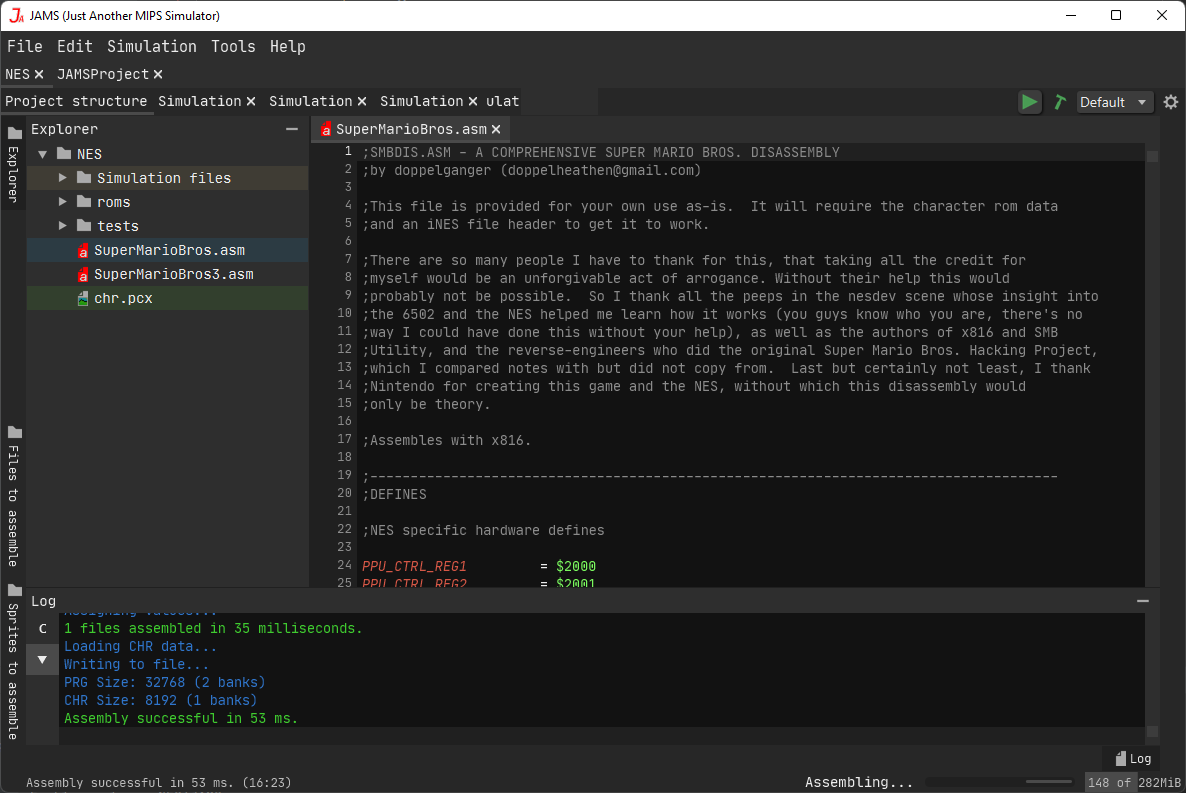
\includegraphics[width=\textwidth]{images/tecnologias/jams-assembling}
    \caption{\textit{JAMS} ejecutando una tarea de ensamblaje}
    \label{fig:jams-assembling}
\end{figure}